\section{Tabellenwerte}
\label{sec:tabelle}
	
	\begin{figure}[H]
		\centering
		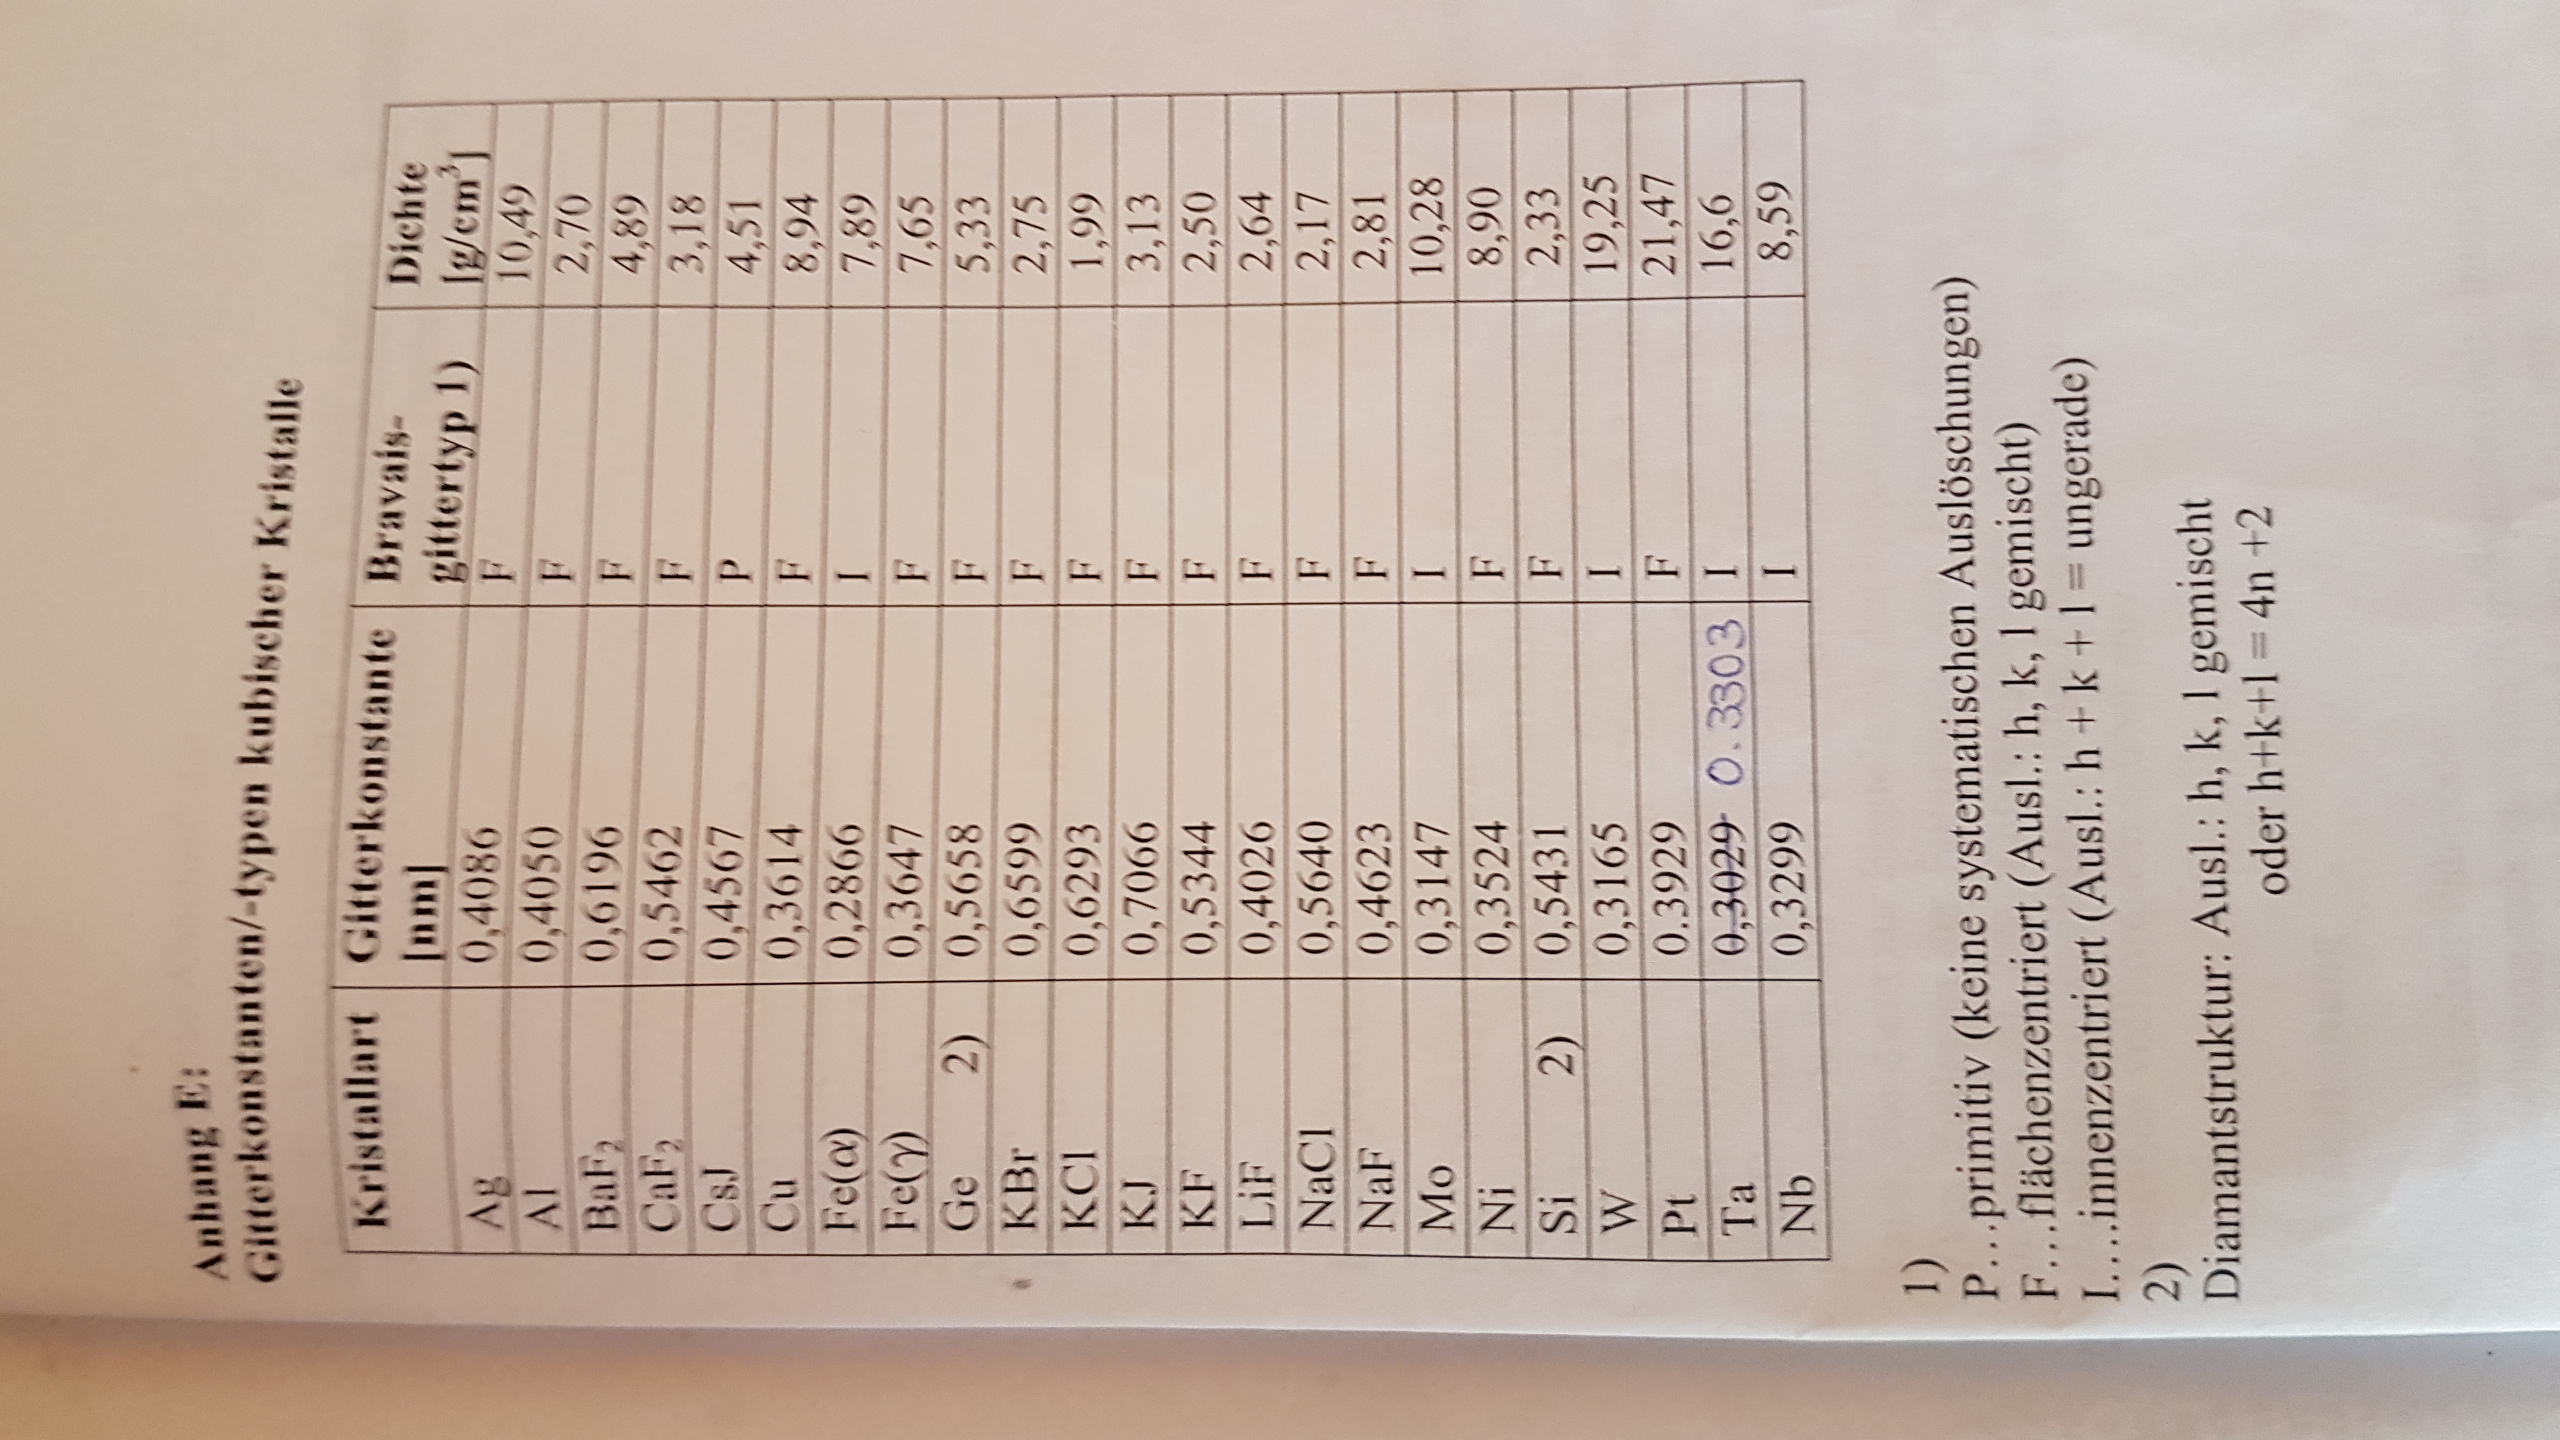
\includegraphics[scale=0.2, angle=-90]{images/20160706_102437.jpg}
		\caption{Tabelle von kristallinen Stoffen mit bekannter Gitterkonstante}
		\label{fig:tab-gitterkonstante}
	\end{figure}

	\begin{figure}[htb]
		\centering
		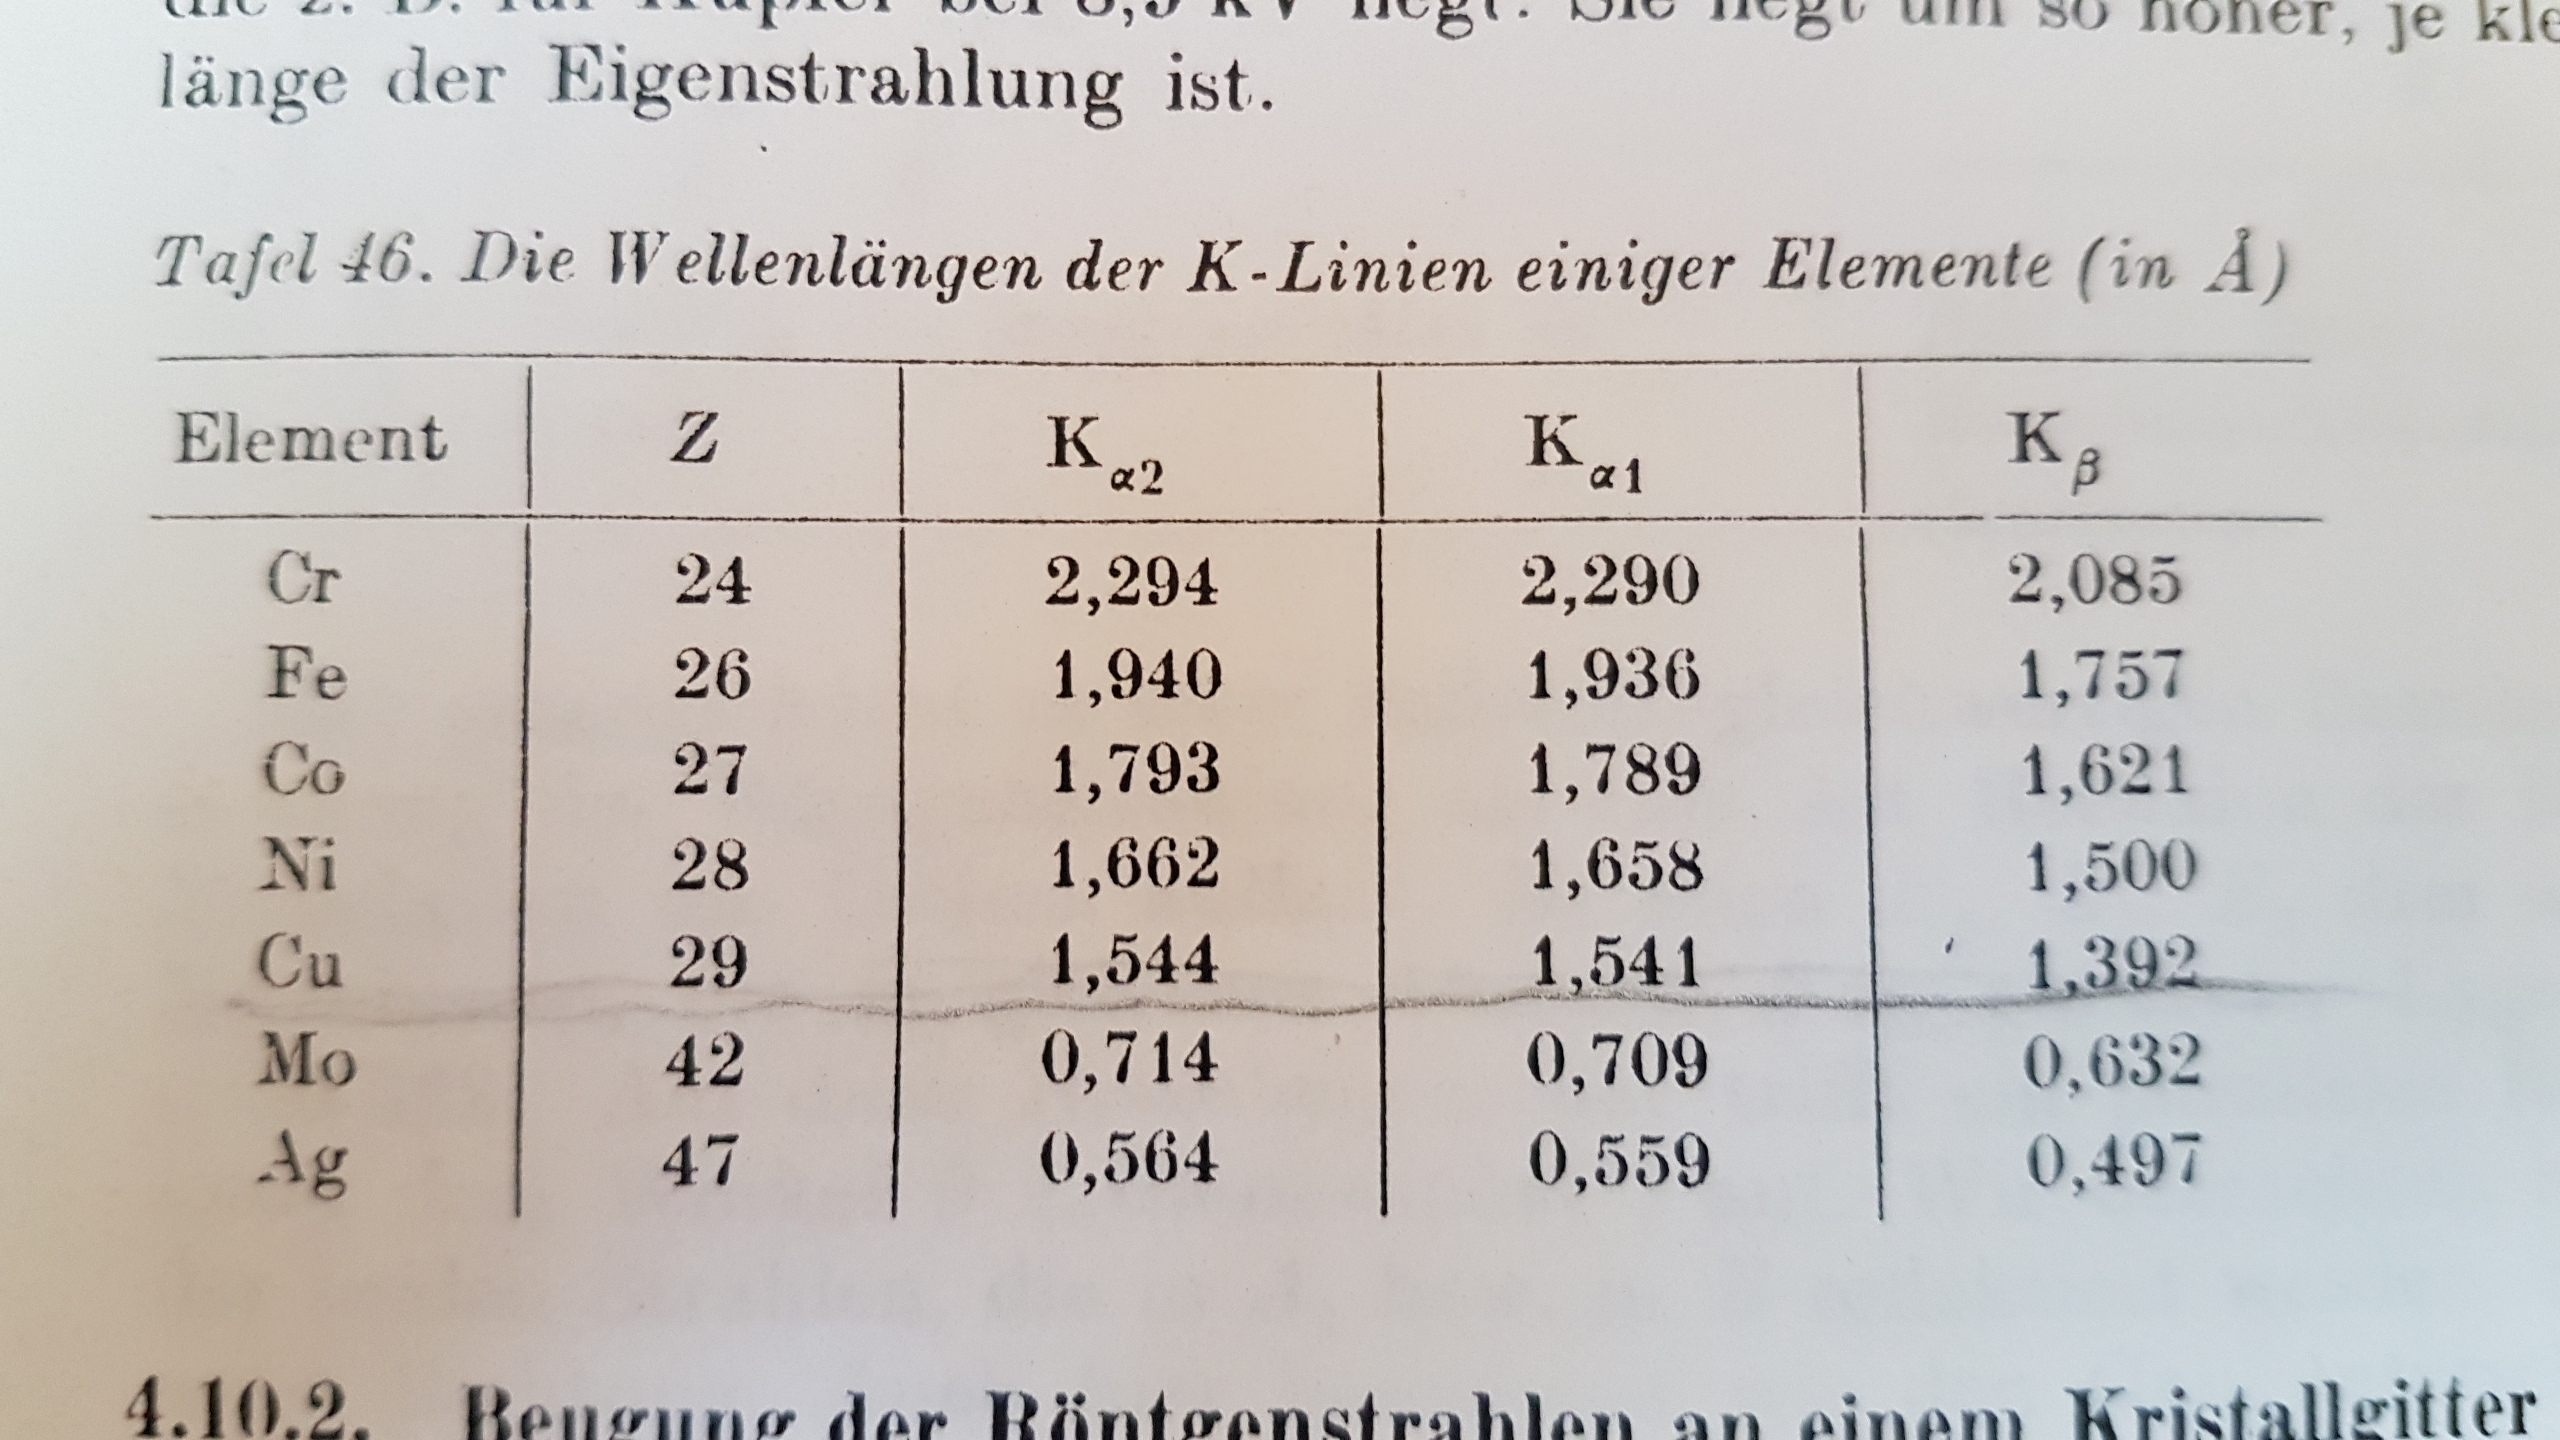
\includegraphics[scale=0.12]{images/lambda-data.jpg}
		\caption{Wellenlängen der K-Linien verschiedener Elemente}
		\label{fig:lambda-data}
	\end{figure}

% section tabelle